%
% \iffalse
%<*driver>
\ProvidesFile{nyu22fonts.dtx}[2023/06/24 v1.4 NYU Typefaces and Fonts]
%</driver>
%<pkg>\ProvidesExplPackage{nyu22fonts}{2023/06/24}{v1.4}{NYU Typefaces and Fonts}
%<*driver>
\documentclass[11pt]{ltxdoc}
\usepackage{dtxdescribe}
\usepackage{graphicx}
\usepackage{changepage}^^A      For the `adjustwidth' environment
\usepackage{hologo}^^A          Provides lots of logos
\usepackage{siunitx}^^A \num, \qty, \ang

\usepackage[backend=biber]{biblatex}
\addbibresource{nyu22fonts.bib}

\usepackage{listings}
\lstset{language=bash,basicstyle=\ttfamily}

\usepackage{titling}
\pretitle{\begin{adjustwidth}{0pt}{-1in}\begin{flushleft}\Huge}
\posttitle{\par\end{flushleft}\end{adjustwidth}\vskip 0.5em}
\predate{\begin{flushleft}}
\postdate{\par\end{flushleft}}
\preauthor{\begin{flushleft}}
\postauthor{\par\end{flushleft}}

\usepackage{xcolor-nyu22}[2022/08/05]
\colorlet{\watchoutcolor}{Magenta}
\usepackage[
    Gotham, Frank Ruhl Libre,
    tone=traditional-subtle]{nyu22fonts}
\linespread{1.041667}
\setmonofont{Inconsolata}

% For documenting expl3 macros, surround the doc element with |\makeusletter|
% and |\makeussubscript|.
\newcommand{\makeusletter}{\catcode`\_=12}
\newcommand{\makeussubscript}{\catcode`\_=8}


\usepackage{parskip}

\renewrobustcmd*{\pkg}[1]{\mbox{\textbf{#1}}}^^A whole document is in sans already
\renewrobustcmd*{\acro}[1]{\MakeUppercase{#1}}^^A Gotham doesn't have small caps
\newcommand{\mtrue}{{\MacroFont true}}
\newcommand{\mfalse}{{\MacroFont false}}
\newcommand{\metatf}{$\left<\mbox{\mtrue}\mid\mbox{\mfalse}\right>$}

\EnableCrossrefs
\RecordChanges
\CodelineIndex
\usepackage{hyperref}
\AtBeginDocument{
  \hypersetup{
    allcolors=NyuViolet,
  }
}
\begin{document}
  \DocInput{nyu22fonts.dtx}
\end{document}
%</driver>
% \fi

% \GetFileInfo{nyu22fonts.dtx} 
% \title{NYU Typefaces and Fonts}
% \author{Matthew Leingang\thanks{leingang@nyu.edu}} \date{\fileversion, Released \filedate}
% \maketitle
%
% \begin{abstract}
%  This package will load fonts for the NYU brand.
%  Package options will allow choices among the primary (proprietary) faces,
%  open (Google) faces, system (Microsoft) faces, and T1 fonts for those who
%  must use \texttt{pdftex}. 
% \end{abstract}
%
% \changes{0.10.4}{2019/12/10}{First working release}
% \changes{0.11.0}{2022/08/16}{Full Implementation of package options}
%
% \tableofcontents
%
% \section{Introduction}
% \begin{refsection}
%
% \subsection{The NYU Typographic Style}
%
% \begin{quotation}
% NYU's typographic language brings your communication to life. Like color, the
% fonts we use reinforce the tone of our communications and designs.
%
% Gotham and Mercury Text are NYU's two typefaces. [See Figures
% \ref{fig-gotham}~and~\ref{fig-mercury-text}.] This versatile group of font
% families can be combined to achieve different tones. That flexibility helps
% our communications appeal to many of our different audiences, including
% students, parents, alumni, faculty and staff, peers, and supporters, while
% maintaining a thematically consistent brand. Font choice also establishes a
% clear hierarchy of information, allowing audiences to easily navigate your
% communications.
%
% \textbf{Gotham} references the no-nonsense signage of New York City. It's a
% typeface that's meant to feel familiar and approachable but strong enough to
% grab and hold your attention within the busy city.
%
% \textbf{Mercury Text} is a high performance serif typeface born from nearly a
% decade of research and development. Mercury Text is resilient enough to work
% in a wide variety of communications.
%
% \hfill---NYU Media and Communications~\cite{nyu-fonts}
% \end{quotation}
%
% \begin{figure}
% 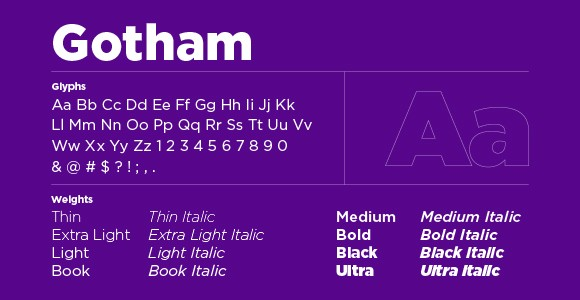
\includegraphics[width=\textwidth]{1645638294211}
% \caption{Gotham and its weights (from~\cite{nyu-fonts})}
% \label{fig-gotham}
% \end{figure}
%
% \begin{figure}
% 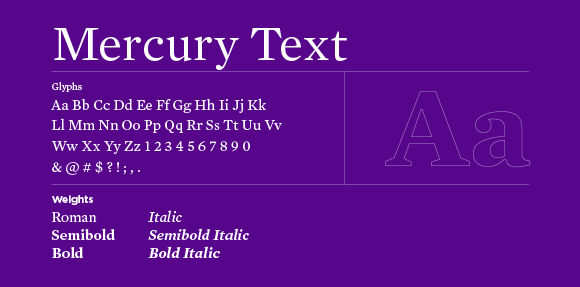
\includegraphics[width=\textwidth]{1645638337298}
% \caption{Mercury Text and its weights (from~\cite{nyu-fonts})}
% \label{fig-mercury-text}
% \end{figure}
%
% \subsection{Setting Visual Tone with Type}
%
% \emph{As above, most this is a paraphrase or direct quote of \cite{nyu-fonts}.
% Visualizations of each tone quadrant are provided there too.}
%
% \subsubsection{Contemporary}
%
% Leverage Gotham's many different weights to create contemporary type
% hierarchies. Gotham is a versatile typeface that can be used in a spectrum
% of ways ranging from subtle to bold and contemporary to traditional. Heavier
% weights of Gotham (like Bold, Black, and Ultra) can generally be used in
% headers to make your communications feel bolder; lighter weights (like Light,
% Book, and Medium) can be used to make your communications feel more subtle.
% Always set body text in Gotham Book for optimal legibility.
%
% \paragraph{Contemporary/Subtle}
% Use lighter weights of Gotham in communications to maintain that contemporary
% edge.
%
% Example: beamer slides from an undergraduate course, an in-class worksheet.
%
% \paragraph{Contemporary/Bold}
% For bolder communications, use heavier weights of Gotham for headlines and
% set them in all caps.
%
% Example: beamer slides for a club presentation.
%
% \subsubsection{Traditional}
%
% Use a combination of Gotham and Mercury to make your communications feel more
% traditional. Since Gotham is our primary typeface, it should always be
% present in our communications. Avoid setting entire communications in Mercury,
% as this starts to feel a bit too traditional and runs the risk of being
% off-brand. In general, consider the typographical balance between your headers
% and body text: if you set your headers in Mercury, use Gotham for body text;
% if you set your headers in Gotham, use Mercury for body text.
%
% \paragraph{Traditional/Subtle}
% Combine Gotham and Mercury for a more traditional visual tone. In subtler
% communications, lighter weights of Gotham can be used as headlines.
%
% Example: lecture notes
%
% \paragraph{Traditional/Bold}
% Use a combination of heavier Gotham weights and Mercury accents to make
% communications feel bold and traditional.
%
% Example: exams.
%
% \subsection{Engines and Font Encodings}
%
% There are several ways a font can be encoded. The ``old'' format is
% PostScript Type~1 or just ``T1''.~\cite{enwiki:1104696616}.  The old format
% is not \emph{as} old as \hologo{TeX}'s native font file format.  Ironically,
% the method for selecting Type~1 fonts in \hologo{TeX} is called the NFSS or
% ``new font selection scheme.''~\cite{texdoc-fntguide}
%
% The ``new'' (still quite old, late 1980s) formats are OpenType (see
% \cite{enwiki:1092758383}) and OpenType. OpenType was built onto OpenType and
% was released in 1996.
%
% There are also several programs, called \emph{engines}, which convert a
% \filenm{.tex} file to a PDF.
%
% Most of the time, the default engine is \hologo{pdfTeX}. This engine only
% handles Type~1 fonts, however. The 21st century engines were designed to
% handle OpenType and OpenType fonts.  \hologo{XeTeX} (first released in 2004)
% also reads input files in unicode rather than plain ASCII, and
% \hologo{LuaTeX} (since 2007) includes a scriptable layer in the lua language.
% The \pkg{fontspec} package~\cite{pkg-fontspec} provides a more modern font
% specification interface.
%
% The upshot is that \textbf{if you want the full features of this package, you
% must use \hologo{XeLaTeX} or \hologo{LuaLaTeX}}. But there are other reasons
% to use them, anyway.  \hologo{LuaTeX} is the engine most in active
% development, so that is the recommended modern engine to adapt.
%
% If you typeset your \filenm{.tex} files on the command line, you just type
% \prog{lualatex} instead of \prog{latex} or \prog{pdflatex}. If you use
% some kind of GUI editor with \hologo{LaTeX} features, search its documentation
% for ``engine'' and you will probably find the option to configure it.

% \section{Installation}

% \subsection{The package}

% To install the package, download the repository and within the module directory,
% execute the command: \prog{l3build install}.

% \subsection{The fonts}
%
% \subsubsection{Gotham}
% 
% To install Gotham, go to \href{https://nyu.onthehub.com/}{OnTheHub} and download
% the zip file of OpenType fonts. Then open the archive and double click on each font.
% It should be added to your system's font library.
%
% \textbf{Note:} Both TrueType and OpenType files can use the \filenm{.ttf} extension.
%
% \subsubsection{Mercury Text}
%
% To install Mercury text, you would need to purchase it directly from
% \href{https://www.typography.com/fonts/mercury-text/styles}{Hoefler\&Co}. 
%
% There \watchout[warning] are pirated OpenType font files purporting to 
% provide various grades of Mercury Text, but they are incorrectly encoded.
% The letters are fine, but several punctuation glyphs are given the wrong
% unicode point. If you install them, your text will be missing quotation marks
% and other punctuation. If you don't want to pay big bucks for Mercury Text,
% settle for Frank Ruhl Libre.
% 
% \subsubsection{Montserrat}
%
% \begin{figure}
% 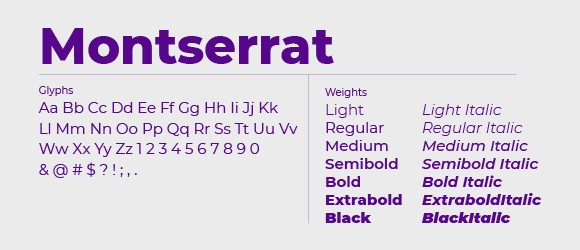
\includegraphics[width=\textwidth]{1645638304749}
% \caption{Montserrat and its weights (from~\cite{nyu-fonts})}
% \label{fig-montserrat}
% \end{figure}
% Montserrat (see Figure~\ref{fig-montserrat}) is a font that is
% included in \hologo{TeX}~Live. So you won't need to install it separately.
% Both Type~1 and OpenType encodings are available.
%
% \subsubsection{Frank Ruhl Libre}
% 
% \begin{figure}
% 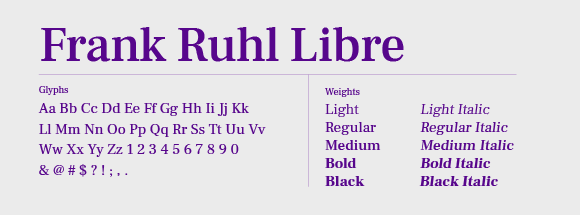
\includegraphics[width=\textwidth]{1645638347113}
% \caption{Frank Ruhl Libre and its weights (from~\cite{nyu-fonts})}
% \label{fig-frl}
% \end{figure}
%
% Frank Ruhl Libre (see Figure~\ref{fig-frl}) is an open licensed OpenType
% font, but it's not in \hologo{TeX}~Live. You can download it from
% \href{https://fonts.google.com/specimen/Frank+Ruhl+Libre}{Google Fonts}.
% Install it by opening the zip file and double-clicking.
%
% \subsubsection{Other Fonts}
%
% The remaining OpenType fonts referenced in this package (Helvetica, Arial,
% Georgia, Times New Roman) should be on your machine already if you have any
% Microsoft or Apple product installed.
%
% The Type~1 fonts referenced will be in \hologo{TeX}~Live.
%
% \section{Usage}
%
% Almost everything in the package is described with keys, as in PGF/TikZ.
% You configure the package using keys in the optional argument to \cs{usepackage},
% as in:
% \begin{sourcedisplay}
% \cs{usepackage}\oarg{keyvals}\{nyu22fonts\}
% \end{sourcedisplay}
%
% \DescribeMacro{\nyufontssetup}
% \cs{nyufontssetup}\marg{keyvals}
% will configure package options after loading, if possible. 
% Some caveats:
% \begin{itemize}
%   \item Some keys require additional packages to be loaded.
%   \item Some keys trigger code to be expanded at the beginning
%     of the document. They won't work after the document begins.  
% \end{itemize}
% These won't work after the document begins.  
%
% \subsection{Setting font families}
%
% Remember that \hologo{XeLaTeX} or \hologo{LuaLaTeX} are required 
% to use OpentType fonts.
% 
% \subsubsection{Setting fonts in groups}
%
% \begin{description}
%
%   \ItemDescribeKey{proprietary} Load Gotham and Mercury Text.
%
%   This option can't be used unless you have \textbf{both}
%   Gotham and Mercury Text. \watchout
%
%   \ItemDescribeKey{open} Load Montserrat and Frank Ruhl Libre.  
%
%   \ItemDescribeKey{system} Load Helvetica and Times New Roman.
%
% \end{description}
%
% \subsubsection{Setting fonts by name}
%
% You can also use the font names themselves as options to the package,
% as in:
% \begin{verbatim}
% \usepackage[Gotham, Frank Ruhl Libre]{nyu22fonts}
% \end{verbatim}
%
% \begin{description}
%   \ItemDescribeKey{Gotham} Use the Gotham family of fonts.
%     To be more precise, this sets:
%     \begin{itemize}
%        \item the default sans font to Gotham Book
%        \item the default bold sans font to Gotham Medium
%        \item the default italic sans font to Gotham Book Italic
%     \end{itemize}
%     The other weights provided in the licensed package are also available
%     using \acro{NFSS} commands:
%     \begin{itemize}
%        \item use \verb|\fontseries{l}\selectfont| to get Gotham Light
%        \item use \verb|\fontseries{l}\selectfont\itshape| to get Gotham Light Italic
%        \item use \verb|\fontseries{b}\selectfont| to get Gotham Bold
%        \item use \verb|\fontseries{b}\selectfont\itshape| to get Gotham Bold Italic
%     \end{itemize}
%
%  \ItemDescribeKey{Mercury Text} Use the Mercury Text G2 family of fonts.
%
%  \ItemDescribeKey{Montserrat} Use the Montserrat family of fonts.
%    This sets:
%    \begin{itemize}
%      \item the default sans font to Montserrat Regular
%      \item the default bold sans font to Montserrat Bold
%      \item the default italic sans font to Montserrat Italic
%    \end{itemize}
%    Like Gotham, Montserrat comes in a variety of weights.
%    These are installed if \pkg{fontspec} is in use.
%    \begin{itemize}
%       \item use \verb|\fontseries{ul}\selectfont| to get Montserrat Thin
%       \item use \verb|\fontseries{el}\selectfont| to get Montserrat Extra Light
%       \item use \verb|\fontseries{l}\selectfont| to get Montserrat Light
%       \item use \verb|\fontseries{sl}\selectfont| to get Montserrat Regular
%       \item use \verb|\fontseries{m}\selectfont| to get Montserrat Medium
%       \item use \verb|\fontseries{sb}\selectfont| to get Montserrat Semi Bold
%       \item use \verb|\fontseries{b}\selectfont| to get Gotham Bold
%       \item use \verb|\fontseries{eb}\selectfont| to get Gotham Extra Bold
%       \item use \verb|\fontseries{ub}\selectfont| to get Gotham Black
%    \end{itemize}
%    Italic shapes are available in all of these weights as well.
%    Juse use \cs{itshape} after selecting the series.
%
%  \ItemDescribeKey{Frank Ruhl Libre} Use the Frank Ruhl Libre family of fonts.
%    This sets:
%    \begin{itemize}
%      \item the default serif or roman font to Frank Ruhl Libre Regular
%      \item the default bold roman font to Frank Ruhl Libre Bold
%      \item the default italic font to a slanted version of Frank Ruhl Libre Regular
%    \end{itemize}
%    The \acro{NFSS} weights are as follows:
%    \begin{itemize}
%       \item use \verb|\fontseries{l}\selectfont| to get Frank Ruhl Libre Light
%       \item use \verb|\fontseries{sl}\selectfont| to get Frank Ruhl Libre Regular
%       \item use \verb|\fontseries{m}\selectfont| to get Frank Ruhl Libre Medium
%       \item use \verb|\fontseries{b}\selectfont| to get Frank Ruhl Libre Bold
%       \item use \verb|\fontseries{eb}\selectfont| to get Frank Ruhl Libre Extra Bold
%    \end{itemize}
%
%  \ItemDescribeKey{Helvetica} Use the Helvetica OpenType family of fonts.
%
%  \ItemDescribeKey{Times New Roman} Use the Times New Roman OpenType family
%    of fonts.
% 
% \end{description}
%
% \subsubsection{Setting fonts automatically}
%
% \DescribeKey{auto}
% Choose the ``best'' available sans and serif fonts. The order of preference
% is proprietary (i.e., Gotham and Mercury Text), open licensed fonts (i.e., 
% Montserrat and Frank Ruhl), then system fonts (i.e., Helvetica and Times New
% Roman). Each font is chosen independently, so you can end up with (for 
% instance) Gotham and Frank Ruhl Libre. 
%
% Use this option with care, because it searches the file system for fonts at
% each \LaTeX{} run. This can slow down your workflow quite a bit.
%
% \subsubsection{\hologo{pdfLaTeX} workarounds}
%
% With the \hologo{pdfTeX} engine, a reasonable attempt is made to imitate
% the desired fonts with available Type~1 alternatives.
%
% \begin{description}
%
%   \ItemDescribeKey{Montserrat} will use the Type~1 encoding of Montserrat.
%
%   \ItemDescribeKey{open} Load Vera Sans and Bitstream Charter.  These are
%     decent open source Type~1 alternatives to Gotham and Mercury Text.
%
%   \ItemDescribeKey{system} Load Type~1 versions of Helvetica and Times New
%     Roman. 
%
% \end{description}
%
% Setting |proprietary| with this engine will \watchout[unavailable key]
% issue a warning, since the proprietary fonts are not available. As a
% fallback, the \PrintDescribeKey{system} key is set instead.
%
% \subsection{Document formatting}
%
% Several keys and meta-keys are used to choose fonts for various document
% elements.
%
% \subsubsection{Formatting document elements}
% \DescribeKey{default family}\meta{font commands}
% This key stores its value in the \cs{familydefault} macro, the default
% document font family. So setting \verb|default family=\sfdefault|
% (for instance) will set the entire document in sans.
%
% \DescribeKey{title/font}\meta{font commands}
% A font hook for the document title and headings. It is initally set to 
% \cs{normalfont}.
%
% \DescribeKey{title/color}\meta{color name}
% A color for the document title and headings. 
% If you set this to |foo|, you are responsible for making sure that
% |\color{foo}| works. This means:
% \begin{itemize}
%   \item The \pkg{color} or \pkg{xcolor} package must be loaded
%   \item The named color |foo| must be defined.
% \end{itemize}
% If the key is unset, the color is not changed from \cs{normalcolor}. 
% The \pkg{xcolor-nyu22} package loads \pkg{xcolor}, adds colors for 
% the brand, and can be used to set this color at package use time:
% \watchout[not implemented]
% \begin{verbatim}
% \usepackage[title/color=NyuViolet]{xcolor-nyu22}
% \end{verbatim}
%
% \DescribeKey{title/uppercase}\metatf, initially \mfalse.
% Set the title in uppercase.
%
% \subsubsection{Setting the document's visual tone}
% 
% \DescribeKey{tone} set the visual tone of the document. The key value
% must be one of the following:
%
% \begin{description}
%   \ItemDescribeKey{contemporary-subtle}
%     Set the default (body) font family to
%     sans, and headers to a lightweight sans.
%   \ItemDescribeKey{contemporary-bold}
%     Set the default font family to sans,
%     and headers to a bold sans. The document title is uppercased.
%   \ItemDescribeKey{traditional-subtle}
%     Set the default font family to sans, section titles to roman.
%   \ItemDescribeKey{traditional-bold}
%     Set the default font family to roman,
%     and headers to a bold sans. 
% \end{description}
%
% \printbibliography[heading=subbibliography]
% \end{refsection}
%
% \StopEventually{\PrintChanges\PrintIndex}
%
% \section{Implementation}
% \begin{refsection}
%
% What follows is the annotated package code. If all you want to do is use the
% package, you can stop reading here.
%
% \makeusletter
%    \begin{macrocode}
%<*pkg>
%    \end{macrocode}
% The package internals are written in the \pkg{expl3} 
% environment.~\cite{pkg-interface3}
%
% \subsection{Messages}
%
%    \begin{macrocode}
\msg_new:nnnn { nyu22fonts } { needsfontspec }{
  Option~`#1'~requires~xelatex~or~lualatex.
}{
  The~option~`#1'~requires~the~xetex~or~luatex~engines~and~
  cannot~be~used~with~pdftex.
}
\msg_new:nnn { nyu22fonts }{ wantsfontspec }{
  For~best~results,~use~xelatex~or~luatex~so~that~OpenType~
  fonts~can~be~used.~Type~1~substitutes~will~be~used~instead.
}
\msg_new:nnn { nyu22fonts }{ substitution }{
  Font~`#2'~unavailable;~substituting~`#1'.
}
\msg_new:nnn { nyu22fonts }{ missingssfont }{
  No~sans~serif~font~found.
}
\msg_new:nnn { nyu22fonts }{ missingsffont }{
  No~serif~font~found.
}
%    \end{macrocode}
%
% Can we use \texttt{fontspec}? If so, load it.
% \changes{v1.2}{2023/06/22}{Drop a global boolean variable and use \cs{IfClassLoadedTF} instead}
%    \begin{macrocode}
\bool_if:nTF { \sys_if_engine_luatex_p: || \sys_if_engine_xetex_p: }
  {
    \RequirePackage{fontspec}
  }
  {
    \msg_warning:nn { nyu22fonts }{ wantsfontspec }
  }
%    \end{macrocode}
%
%
% \subsection{Font specification commands}
%
% \subsubsection{Proprietary fonts}
%
% \begin{macro}{\__nyufonts_set_gotham:}
% \changes{v1.1}{2023/06/19}{Assign all available (licensed) weights to \acro{NFSS} series}
% Set the default sans family to Gotham.
% \changes{v1.2}{2023/06/21}{Raise an error if \pkg{fontspec} is unavailable, fall back to Helvetica}
%
% We use both the \pkg{fontspec} and \acro{NFSS} methods for choosing font
% faces, so that we can assign all the weights provided in the licensed
% package. We reserve space in the \acro{NFSS} weight spectrum for the other
% known, but possibly not installed, weights. Unlicensed versions of these can
% be found online, but using them is trickier and may be engine-dependent.
% Use at your own risk.
%
% \begin{tabular}{llll}
%     Official weight & \acro{NFSS} weight & licensed & unlicensed \\
%     \hline
%     Thin            & \texttt{ul}        & No       & Yes \\
%     XLight          & \texttt{el}        & No       & Yes \\
%     Light           & \texttt{l}         & Yes      & Yes \\
%     Book            & \texttt{m}         & Yes      & Yes \\
%     Medium          & \texttt{sb}        & Yes      & Yes \\
%     Bold            & \texttt{b}         & Yes      & Yes \\
%     Black           & \texttt{eb}        & No       & upright only \\
%     Ultra           & \texttt{ub}        & No       & italic only
% \end{tabular}
%
% The default “boldface” series is set to \texttt{sb}, which is mapped to 
% Gotham Medium. 
% 
%    \begin{macrocode}
\cs_new:Nn \__nyufonts_set_gotham: {
  \IfPackageLoadedTF{fontspec}{
    \setsansfont{Gotham}[
      FontFace={l}{n}{*~Light},
      FontFace={l}{it}{*~Light~Italic},
      FontFace={sb}{n}{*~Medium},
      FontFace={sb}{it}{*~Medium~Italic},
      FontFace={b}{n}{*~Bold},
      FontFace={b}{it}{*~Bold~Italic},
      UprightFont=*~Book,
      BoldFont=*~Medium,
      ItalicFont=*~Book~Italic,
      BoldItalicFont=*~Medium~Italic
    ]
  }
  {
    \msg_error:nnn { nyu22fonts } { needsfontspec } { Gotham } 
    \msg_warning:nnnn { nyu22fonts } { substitution } { Montserrat~Type~1 } { Gotham }
    \usepackage{montserrat}
  }
}
%    \end{macrocode}  
% \end{macro}
%
% \begin{macro}{\__nyufonts_set_mercury_text:}
% \changes{v1.2}{2023/06/21}{Raise an error if \pkg{fontspec} is unavailable, fall back to Charter}
% Set the default roman family to Mercury Text Grade~2.
%    \begin{macrocode}
\cs_new:Nn \__nyufonts_set_mercury_text: {
  \IfPackageLoadedTF{fontspec}{
    \setmainfont{Mercury~Text~G2}[
      UprightFont=*~Roman,
      BoldFont=*~Bold,
      ItalicFont=*~Italic
    ]
  }
  {
    \msg_error:nnn { nyu22fonts } { needsfontspec } { Mercury~Text }
    \msg_warning:nnnn { nyu22fonts } { substitution } { Charter } { Mercury~Text }
    \__nyufonts_set_charter:
  }
}
%    \end{macrocode}  
% \end{macro}
%
% \subsubsection{Open fonts}
%
% \begin{macro}{\__nyufonts_set_montserrat:}
% \changes{v1.1}{2023/06/20}{Assign all available weights to \acro{NFSS} series}
% \changes{v1.2}{2023/06/21}{If \pkg{fontspec} is unavailable, fall back to the non-fontspec version}
% Set the default sans family to Montserrat. There is already a
% \pkg{montserrat} package with a \filenm{montserrat.fontspec} file, but we
% want to use all the available weights.
%
% \begin{tabular}{lll}
%     Official weight & \acro{NFSS} weight & \acro{NFSS} series \\
%     \hline
%     Thin            & Ultra Light        & \texttt{ul}      \\
%     ExtraLight      & Extra Light        & \texttt{el}      \\
%     Light           & Light              & \texttt{l}       \\
%     Regular         & Semi Light         & \texttt{sl}      \\
%     Medium          & Medium             & \texttt{m}       \\
%     SemiBold        & Semi Bold          & \texttt{sb}      \\
%     Bold            & Bold               & \texttt{b}       \\
%     ExtraBold       & Extra Bold         & \texttt{eb}      \\
%     Black           & Ultra Bold         & \texttt{ub}   
% \end{tabular}
%
% After setting these, the default medium series weight is set to Regular,
% and the default bold series weight to semibold. This seems to match the
% pairing of Gotham Book and Medium.
%    \begin{macrocode}
\cs_new:Nn \__nyufonts_set_montserrat: {
  \IfPackageLoadedTF{fontspec}{
    \setsansfont{Montserrat}[
      Extension = .otf,
      FontFace={ul}{n}{*-Thin},
      FontFace={ul}{it}{*-ThinItalic},    
      FontFace={el}{n}{*-ExtraLight},
      FontFace={el}{it}{*-ExtraLightItalic},    
      FontFace={l}{n}{*-Light},
      FontFace={l}{it}{*-LightItalic},    
      FontFace={sl}{n}{*-Regular},
      FontFace={sl}{it}{*-Italic},    
      FontFace={m}{n}{*-Medium},
      FontFace={m}{it}{*-MediumItalic},    
      FontFace={sb}{n}{*-SemiBold},
      FontFace={sb}{it}{*-SemiBold},    
      FontFace={b}{n}{*-Bold},
      FontFace={b}{it}{*-BoldItalic},    
      FontFace={eb}{n}{*-ExtraBold},
      FontFace={eb}{it}{*-ExtraBoldItalic},    
      FontFace={ub}{n}{*-Black},
      FontFace={ub}{it}{*-BlackItalic},    
      UprightFont = *-Regular ,
      ItalicFont = *-Italic ,
      BoldFont = *-SemiBold ,
      BoldItalicFont = *-SemiBoldItalic ,
    ]
  }{
    \msg_warning:nnnn { nyu22fonts } { substitution } 
      { Montserrat~Type~1 } { Montserrat~OpenType }
    \usepackage{montserrat}
  }
}
%    \end{macrocode}
% \end{macro}
%
% \begin{macro}{\__nyufonts_set_frank_ruhl_libre:}
% \changes{v0.14h}{2023/06/12}{Don't also set the sans font simultaneously.}
% \changes{v1.1}{2023/06/20}{Assign all available weights}
% \changes{v1.2}{2023/06/21}{Raise an error if \pkg{fontspec} is unavailable, fall back to Charter}
% Set the default roman family to Frank Ruhl Libre.
% We assign all the weights available in the Google Font download package.
%
% \begin{tabular}{lll}
%     Official weight & \acro{NFSS} weight & \acro{NFSS} series \\
%     \hline
%     Light           & Light              & \texttt{l}       \\
%     Regular         & Semi Light         & \texttt{sl}      \\
%     Medium          & Medium             & \texttt{m}       \\
%     Bold            & Bold               & \texttt{b}       \\
%     Black           & Extra Bold         & \texttt{eb}   
% \end{tabular}
%  
% Note that there are no open-licensed italic fonts for this family. NYU
% \cite{nyu-fonts} says to skew the upright font by \ang{14}. We use
% \pkg{fontspec} options to fake it. 
%
% \begin{macro}{\g__nyufonts_slant_fp:}
% \changes{v1.1}{2023/06/20}{Add this variable to match specified skew}
% The argument to \PrintDescribeKey{FakeSlant} is apparently (see 
% \cite{ctt-fakeslant}) the ratio of horizontal skew to vertical distance. 
% We use $\tan(\ang{14}) \approx \num{0.24932800284}$.
% 
%    \begin{macrocode}
\fp_new:N  \g__nyufonts_slant_fp:
\fp_gset:Nn \g__nyufonts_slant_fp: { 0.24932800284 }
%    \end{macrocode}
% \end{macro}
% 
%    \begin{macrocode}
\cs_new:Nn \__nyufonts_set_frank_ruhl_libre: {
  \IfPackageLoadedTF{fontspec}{
    \setmainfont{Frank~Ruhl~Libre}[
      FontFace={l}{n}{*~Light},
      FontFace={l}{it}{Font=*~Light,FakeSlant=\fp_use:N \g__nyufonts_slant_fp:},
      FontFace={sl}{n}{*~Regular},
      FontFace={sl}{it}{Font=*~Regular,FakeSlant=\fp_use:N \g__nyufonts_slant_fp:},
      FontFace={m}{n}{*~Medium},
      FontFace={m}{it}{Font=*~Medium,FakeSlant=\fp_use:N \g__nyufonts_slant_fp:},
      FontFace={b}{n}{*~Bold},
      FontFace={b}{it}{Font=*~Bold,FakeSlant=\fp_use:N \g__nyufonts_slant_fp:},
      FontFace={eb}{n}{*~Black},
      FontFace={eb}{it}{Font=*~Black,FakeSlant=\fp_use:N \g__nyufonts_slant_fp:},
      UprightFont=*,
      ItalicFont=*,
      ItalicFeatures={FakeSlant=\fp_use:N \g__nyufonts_slant_fp:},
      BoldItalicFont=*~Bold,
      BoldItalicFeatures={FakeSlant=\fp_use:N \g__nyufonts_slant_fp:},
    ]
  }{
    \msg_error:nnn { nyu22fonts } { needsfontspec } { Frank~Ruhl~Libre }
    \__nyufonts_set_charter:
  }
}
%    \end{macrocode}
% \end{macro}
%
% \subsubsection{\LaTeX{} Type~1 approximations}
% 
% These are not official font options but pretty good approximations to
% the official open ones.
% 
% \begin{macro}{\__nyufonts_set_vera:}
% Set the default sans family to Vera. The mono family is set to Bera, 
% but the roman family is left alone.
% \changes{v0.11c}{2022/10/01}{Fix a bug introduced by the \pkg{arev} package also setting the \emph{serif} font.}
%    \begin{macrocode}
\cs_new:Nn \__nyufonts_set_vera: {
  \RequirePackage[T1]{fontenc}
  \RequirePackage{textcomp}
  \renewcommand{\sfdefault}{fav}
  \renewcommand{\ttdefault}{fvm}
  \RequirePackage{arevmath}
  \RequirePackage{beramono}
}
%    \end{macrocode}  
% \end{macro}
%
% \begin{macro}{\__nyufonts_set_charter:}
% Set the default roman family to Charter.
%    \begin{macrocode}
\cs_new:Nn \__nyufonts_set_charter: {
  \RequirePackage{charter}
}
%    \end{macrocode}  
% \end{macro}
%
%
% \subsubsection{System Fonts}
%
% \begin{macro}{\__nyufonts_set_helvetica_tt:}
% Set the default sans family to the OpenType Helvetica font.
%    \begin{macrocode}
\cs_new:Nn \__nyufonts_set_helvetica_tt: {
  \setsansfont{Helvetica}
}
%    \end{macrocode}
% \end{macro}
%
% \begin{macro}{\__nyufonts_set_times_new_roman_tt:}
% Set the default roman family to the OpenType Times New Roman font.
%    \begin{macrocode}
\cs_new:Nn \__nyufonts_set_times_new_roman_tt: {
  \setmainfont{Times~New~Roman}
}
%    \end{macrocode}
% \end{macro}
%
% \subsubsection{Type 1 fonts}
%
% \begin{macro}{\__nyufonts_set_helvetica_ti:}
% Set the default sans family to the Type~1 version of Helvetica.
% (Technically, not Helvetica, but a Type~1 clone called Nimbus Sans.)
%    \begin{macrocode}
\cs_new:Nn \__nyufonts_set_helvetica_ti: {
  \usepackage{helvet}
}
%    \end{macrocode}
% \end{macro}
%
% \begin{macro}{\__nyufonts_set_times_new_roman_ti:}
% Set the default roman family to the Type~1 version of Times New Roman.
%    \begin{macrocode}
\cs_new:Nn \__nyufonts_set_times_new_roman_ti: {
  \usepackage{mathptmx}
}
%    \end{macrocode}
% \end{macro}
%
%  
% \subsection{Selecting fonts automatically}
%
% \begin{macro}{\__nyufonts_auto_select_ss_font:}
% Choose the sans serif font automatically.
%    \begin{macrocode}
\cs_new:Nn \__nyufonts_auto_select_ss_font: {
  \IfPackageLoadedTF{fontspec}{
    \fontspec_font_if_exist:nTF { Gotham~Book } {
      \__nyufonts_set_gotham:
    }{
      \fontspec_font_if_exist:nTF { Montserrat } {
        \__nyufonts_set_montserrat:
      }{
        \fontspec_font_if_exist:nTF { Helvetica } {
          \__nyufonts_set_helvetica_tt:
        }{
          \msg_error:nn { nyu22fonts }{ missingssfont }
        }
      }
    }
  }{
    \__nyufonts_set_vera:
  }
}
%    \end{macrocode}
% \end{macro}
%
% \begin{macro}{\__nyufonts_auto_select_sf_font:}
% Choose the serif font automatically.
%    \begin{macrocode}
\cs_new:Nn \__nyufonts_auto_select_sf_font: {
  \IfPackageLoadedTF{fontspec}{
    \fontspec_font_if_exist:nTF { Mercury~Text~G2~Roman } {
      \__nyufonts_set_mercury_text:
    }{
      \fontspec_font_if_exist:nTF { Frank~Ruhl~Libre } {
        \__nyufonts_set_frank_ruhl_libre:
      }{
        \fontspec_font_if_exist:nTF { Times~New~Roman } {
          \__nyufonts_set_helvetica_tt:
        }{
          \msg_error:nn { nyu22fonts }{ missingsffont }
        }
      }
    }
  }{
    \__nyufonts_set_charter:
  }
}
%    \end{macrocode}  
% \end{macro}
% 
% \subsection{Document formatting}
%
% \begin{key}{default family}
% \changes{v1.3}{2023/06/23}{Provide this key} 
%    \begin{macrocode}
\keys_define:nn { nyufonts } {
  default~family .tl_set:N = \familydefault
}
%    \end{macrocode}
% \end{key}

%
% \begin{hook}{\l__nyufonts_title_font_tl}
% \changes{v1.3}{2023/06/22}{Add this variable}
% A hook for setting the fonts of titles.
%    \begin{macrocode}
\tl_new:N \l__nyufonts_title_font_tl
\tl_set:Nn \l__nyufonts_title_font_tl \normalfont
%    \end{macrocode}
% \end{hook}
% 
% \begin{key}{title/font}
% \changes{v1.3}{2023/06/23}{Add this key}
% Store the title font.
%    \begin{macrocode}
\keys_define:nn { nyufonts } {
  title/font .tl_set:N = { \l__nyufonts_title_font_tl }
}
%    \end{macrocode}
% \end{key}
%
% \begin{macro}{\l__nyucolors_title_color_tl}
% \changes{v1.3}{2023/06/22}{Provide this variable}
% A hook for setting the color of titles. The \pkg{xcolor-nyu22} package can be
% used to change this to something else.
%    \begin{macrocode}
\tl_if_exist:NF \l__nyucolors_title_color_tl { 
  \tl_new:N \l__nyucolors_title_color_tl
}
%    \end{macrocode}
% \end{macro}
% \begin{key}{title/color}
% \changes{v1.3}{2023/06/23}{Provide this key}
% \changes{v1.4}{2023/06/24}{Migrate to this module's namespace}
% \changes{v1.4}{2023/06/24}{Refer to a color name instead of a color hook}
% Store the title color. 
% The \pkg{xcolor-nyu22} package may also set this key.
%    \begin{macrocode}
\keys_define:nn { nyufonts } {
  title/color .tl_set:N = { \l__nyucolors_title_color_tl }
}
%    \end{macrocode}
% \end{key}
%
% \begin{macro}{\l__nyufonts_title_uppercase_bool}
% \begin{key}{title/uppercase}
% \changes{v1.3}{2023/06/23}{Provide this key}
% When true, set the title in upper case.
%    \begin{macrocode}
\keys_define:nn { nyufonts } {
  title/uppercase .bool_set:N = \l__nyufonts_title_uppercase_bool
}
%    \end{macrocode}
% \end{key}
% \end{macro}
%
%
% \begin{macro}{\l__nyufonts_reset_title_bool}
% \changes{v1.3}{2023/06/23}{Added this variable}
% If true, reset the title with the \pkg{titling} package.
% The initial value is \verb|true| unless we're using the 
% \cls{beamer} class and not ``article mode''.
% 
%    \begin{macrocode}
\bool_new:N \l__nyufonts_reset_title_bool
\IfPackageLoadedTF{beamerarticle}{
  \bool_set_true:N \l__nyufonts_reset_title_bool    
}{
  \IfClassLoadedTF{beamer}{
    \bool_set_false:N \l__nyufonts_reset_title_bool    
  }{
    \cs_if_exist:NT \maketitle {
      \bool_set_true:N \l__nyufonts_reset_title_bool 
    }{
      \bool_set_false:N \l__nyufonts_reset_title_bool
    }
  }
}
%    \end{macrocode}
% \end{macro}
%
% \begin{macro}{\__nyufonts_reset_article_title:}
% Reset the article title, inserting the title font and color.
% \changes{v1.3}{2023/06/23}{Add this function} 
%    \begin{macrocode}
\cs_new:Nn \__nyufonts_use_color_if_exist:N {
  \tl_if_eq:NNF #1 \c_empty_tl {
    \color{#1}
  }
}
\cs_new:Nn \__nyufonts_reset_title: {
  \RequirePackage{titling}
  \pretitle{\begin{flushleft}
    \__nyufonts_use_color_if_exist:N \l__nyucolors_title_color_tl
    \l__nyufonts_title_font_tl
    \bool_if:NT \l__nyufonts_title_uppercase_bool {
      \tl_set:cx {@title} { \text_uppercase:n { \tl_use:c {@title} } }
    }\Huge}
  \posttitle{\par\end{flushleft}\vskip 0.5em}
  \predate{\begin{flushleft}
    \__nyufonts_use_color_if_exist:N \l__nyucolors_title_color_tl
    \l__nyufonts_title_font_tl
    \large}
  \postdate{\par\end{flushleft}}
  \preauthor{\begin{flushleft}
    \__nyufonts_use_color_if_exist:N \l__nyucolors_title_color_tl
    \l__nyufonts_title_font_tl
    \large}
  \postauthor{\par\end{flushleft}}
}
%    \end{macrocode}
% We do this when the boolean is set.
%    \begin{macrocode}
\AtBeginDocument{
  \bool_if:NT \l__nyufonts_reset_title_bool \__nyufonts_reset_title:
}
%    \end{macrocode}
% \end{macro}
%
% \begin{macro}{\l__nyufonts_reset_headers_bool}
% \changes{v1.3}{2023/06/23}{Add this variable}
% If true, reset the header titles with the \pkg{titlesec} package.
%    \begin{macrocode}
\bool_new:N \l__nyufonts_reset_headers_bool
\bool_set_eq:NN \l__nyufonts_reset_headers_bool \l__nyufonts_reset_title_bool
%    \end{macrocode}
% \end{macro}
%
% \begin{macro}{\__nyufonts_reset_headers:}
% \changes{v1.3}{2023/06/23}{Add this function} 
%    \begin{macrocode}
\cs_set:Nn \__nyufonts_reset_headers: {
  \RequirePackage{titlesec}
  \titleformat*{\section}{
    \__nyufonts_use_color_if_exist:N \l__nyucolors_title_color_tl
    \l__nyufonts_title_font_tl
    \LARGE}
  \titleformat*{\subsection}{
    \__nyufonts_use_color_if_exist:N \l__nyucolors_title_color_tl
    \l__nyufonts_title_font_tl
    \Large}
  \titleformat*{\subsubsection}{
    \__nyufonts_use_color_if_exist:N \l__nyucolors_title_color_tl
    \l__nyucolors_title_color_tl
    \l__nyufonts_title_font_tl
    \large}
    \titleformat*{\paragraph}{
      \__nyufonts_use_color_if_exist:N \l__nyucolors_title_color_tl
      \l__nyucolors_title_color_tl
      \l__nyufonts_title_font_tl
      \normalsize}
  }
%    \end{macrocode}
% We do this when the boolean is set.
%    \begin{macrocode}
\AtBeginDocument{
  \bool_if:NT \l__nyufonts_reset_headers_bool \__nyufonts_reset_headers:
}
%    \end{macrocode}
% \end{macro}
%
% \begin{macro}{\g__nyufonts_doc_is_booklike_bool,\g__nyufonts_doc_is_articlelike_bool}
%   The standard classes \cls{book} and \cls{report} are
%   divided into chapters by the \cs{chapter} command.
%   But \cls{articles} only have \cs{section}s.
%
%   Today I learned that \cs{IfClassLoadedTF} exists, but I'm going to 
%   use duck typing here.
%    \begin{macrocode}
\bool_new:N \g__nyufonts_doc_is_booklike_bool
\bool_gset_false:N \g__nyufonts_doc_is_booklike_bool
\bool_new:N \g__nyufonts_doc_is_articlelike_bool
\bool_gset_false:N \g__nyufonts_doc_is_articlelike_bool
\cs_if_exist:NT \section {
  \cs_if_exist:NTF \chapter {
    \bool_gset_true:N \g__nyufonts_doc_is_booklike_bool
  }{
    \bool_gset_true:N \g__nyufonts_doc_is_articlelike_bool
  }
}
%    \end{macrocode}
% \end{macro}
%
%
% \begin{macro}{\__nyufonts_set_tone_cs:}
% \changes{v1.2a}{2023/06/22}{Set heading font to sans light, per specification}
%   Set the document's visual tone to Contemporary/Subtle:
%   \begin{itemize}
%     \item Default (body) family sans
%     \item Headers in a light sans
%   \end{itemize}
% 
%    \begin{macrocode}
\cs_new:Nn \__nyufonts_set_headers: {

}
\cs_new:Nn \__nyufonts_set_tone_cs: {
  \renewcommand{\familydefault}{\sfdefault}
  \renewcommand{\l__nyufonts_title_font_tl}{\sffamily\fontseries{l}\selectfont}
  \bool_if:NT \g__nyufonts_doc_is_articlelike_bool {
    \__nyufonts_set_article_title:
    \RequirePackage{titlesec}
    \titleformat*{\section}{\LARGE\l__nyufonts_title_font_tl}
    \titleformat*{\subsection}{\Large\l__nyufonts_title_font_tl}
    \titleformat*{\subsubsection}{\large\l__nyufonts_title_font_tl}
  }
}
%    \end{macrocode}
% \end{macro}
%
% \begin{macro}{\__nyufonts_set_tone_cb:}
% \changes{v1.3}{2023/06/22}{Added implementation}
%   Set the document's visual tone to Contemporary/Bold:
%   \begin{itemize}
%     \item Default (body) family sans
%     \item Headers bold and sometimes uppercased
%   \end{itemize}
% 
%    \begin{macrocode}
\cs_new:Nn \__nyufonts_set_tone_cb: {
  \renewcommand{\familydefault}{\sfdefault}
  \renewcommand{\l__nyufonts_title_font_tl}{\sffamily\fontseries{b}\selectfont}
  \bool_if:NT \g__nyufonts_doc_is_articlelike_bool {
    \RequirePackage{titling}
    \pretitle{\begin{flushleft}%
      \edef\@TITLE{\MakeUppercase{\@title}}%
      \let\@title\@TITLE
      \l__nyufonts_title_font_tl\Huge}
    \posttitle{\par\end{flushleft}\vskip 0.5em}
    \predate{\begin{flushleft}}
    \postdate{\par\end{flushleft}}
    \preauthor{\begin{flushleft}}
    \postauthor{\par\end{flushleft}}
    \RequirePackage{titlesec}
    \titleformat*{\section}{\LARGE\l__nyufonts_title_font_tl}
    \titleformat*{\subsection}{\Large\l__nyufonts_title_font_tl}
    \titleformat*{\subsubsection}{\large\l__nyufonts_title_font_tl}
  }
}
%    \end{macrocode}
% \end{macro}
%
%
% \section{Keyval interface}
%
% The main processing is done with a keyval interface.
% \changes{v0.15}
%  {2023/06/12}
%  {Fix a bug wherein spaces in option values were ignored}
%    \begin{macrocode}
\keys_define:nn { nyufonts }
  {
    proprietary .meta:n = { font-group = proprietary },
    open .meta:n = { font-group = open },
    system .meta:n = { font-group = system},
    auto .code:n = { 
      \__nyufonts_auto_select_sf_font:
      \__nyufonts_auto_select_ss_font:
    },

    serif-font .choice:,
    serif-font / Mercury~Text           .code:n = { \__nyufonts_set_mercury_text: },
    serif-font / Frank~Ruhl~Libre       .code:n = { \__nyufonts_set_frank_ruhl_libre:}, 
    serif-font / Charter                .code:n = { \__nyufonts_set_charter:},
    serif-font / Charter                .usage:n = preamble,
    serif-font / Times~New~Roman~Type~1 .code:n = { \__nyufonts_set_times_new_roman_ti: },
    serif-font / Times~New~Roman~Type~1 .usage:n = preamble,
    serif-font / Times~New~Roman~OpenType .code:n = { \__nyufonts_set_times_new_roman_tt: },

    sans-serif-font .choice:,
    sans-serif-font / Gotham           .code:n = { \__nyufonts_set_gotham: },
    sans-serif-font / Montserrat       .code:n = { \__nyufonts_set_montserrat: },
    sans-serif-font / Helvetica~Type~1 .code:n = { \__nyufonts_set_helvetica_ti: },
    sans-serif-font / Helvetica~Type~1 .usage:n = preamble,
    sans-serif-font / Helvetica~OpenType .code:n = {\__nyufonts_set_helvetica_tt: },
    sans-serif-font / Vera             .code:n = { \__nyufonts_set_vera: },
    sans-serif-font / Vera             .usage:n = preamble,
%    \end{macrocode}
%
% \begin{key}{Gotham}
% \changes{v0.14h}{2023/06/12}{Added Gotham and Frank Ruhl Libre meta-keys}
% Set Gotham.
%    \begin{macrocode}
    Gotham .meta:n = { sans-serif-font = Gotham }, 
%    \end{macrocode}
% \end{key}
% \begin{key}{Frank Ruhl Libre}
% Set Frank Ruhl Libre.
%    \begin{macrocode}
    Frank~Ruhl~Libre .meta:n = { serif-font = Frank~Ruhl~Libre },
%    \end{macrocode}
% \end{key}  
%
% \changes{v0.16}{2023/06/12}{Added the rest of the OpenType fonts as meta-keys}
%    \begin{macrocode}
    Montserrat .meta:n = { sans-serif-font = Montserrat }, 
    Helvetica .meta:n = { sans-serif-font = Helvetica~OpenType }, 

    Mercury~Text .meta:n = { serif-font = Mercury~Text},
    Times~New~Roman .meta:n = { serif-font = Times~New~Roman~OpenType},

    font-group .choice:,
    font-group / proprietary .code:n = {
      \IfPackageLoadedTF{fontspec}{
        \__nyufonts_set_gotham:
        \__nyufonts_set_mercury_text:
      }{
        \msg_error:nnn { nyu22fonts } { needsfontspec } { proprietary }
        \__nyufonts_set_helvetica_ti:
        \__nyufonts_set_times_new_roman_ti:
      }
    },
    font-group / open .code:n = {
      \IfPackageLoadedTF{fontspec}{
        \__nyufonts_set_montserrat:
        \__nyufonts_set_frank_ruhl_libre:
      }{
        \__nyufonts_set_vera:
        \__nyufonts_set_charter:
      }
    },
    font-group / system .code:n = {
      \IfPackageLoadedTF{fontspec}{
        \__nyufonts_set_helvetica_tt:
        \__nyufonts_set_times_new_roman_tt:
      }{
        \__nyufonts_set_helvetica_ti:
        \__nyufonts_set_times_new_roman_ti:
      }
    },
    font-group .initial:n = system,

%    \end{macrocode}
% \begin{key}{tone}
%    \begin{macrocode}
    tone .choice:,
%    \end{macrocode}
% \end{key}
%
% \begin{key}{tone/contemporary-subtle}
%    \begin{macrocode}
    tone/contemporary-subtle .meta:n = {
      default~family=\sfdefault, 
      title/font=\sffamily\fontseries{l}\selectfont,
    },
%    \end{macrocode}  
% \end{key}
% \begin{key}{contemporary-bold}
%    \begin{macrocode}
    tone/contemporary-bold .meta:n = {
      default~family=\sfdefault, 
      title/font=\sffamily\fontseries{b}\selectfont,
      title/uppercase,
    },
%    \end{macrocode}  
% \end{key}
% \begin{key}{traditional-subtle}
%    \begin{macrocode}
    tone/traditional-subtle .meta:n = {
      default~family=\sfdefault, 
      title/font=\rmfamily\fontseries{m}\selectfont,
    },
%    \end{macrocode}  
% \end{key}
% \begin{key}{traditional-bold}
%    \begin{macrocode}
    tone/traditional-bold .meta:n = {
      default~family=\rmdefault, 
      title/font=\sffamily\fontseries{b}\selectfont,
      title/uppercase=false,
    },
%    \end{macrocode}  
% \end{key}
%
% End of the \cs{keys_define} group.
%    \begin{macrocode}
  }
%    \end{macrocode}
% \makeussubscript
%
% Process keyval options provided with \cs{usepackage}.
% The \pkg{l3keys2e} package is obsolete with the June 2022 \LaTeX{} release.
% See~\cite{tse-l3keys2e}.
%    \begin{macrocode}
\IfFormatAtLeastTF { 2022-06-01 }
{ 
  \ProcessKeyOptions [ nyufonts ]
}{
  \RequirePackage { l3keys2e }
  \ProcessKeysOptions { nyufonts }
}  
%
%    \end{macrocode}
%
% \begin{macro}{\nyufontssetup}
% Set keyval options after package loading.
%    \begin{macrocode}
\newcommand{\nyufontssetup}[1]{
  \IfFormatAtLeastTF { 2022-06-01 }
  { 
    \SetKeys[ nyufonts ]{#1} 
  }{  
    \keys_set:nn { nyufonts }{ #1 } 
  }  
}
%    \end{macrocode}
% \end{macro}
%
%    \begin{macrocode}
%</pkg>
%    \end{macrocode}
%
% \printbibliography[
%   heading=subbibliography,
%   title={Implementation References}]
% \end{refsection}
%
% \Finale
